\subsection{The EBIT method}

% ----------
\begin{figure}
\begin{center}
\begin{tabular}{cc}
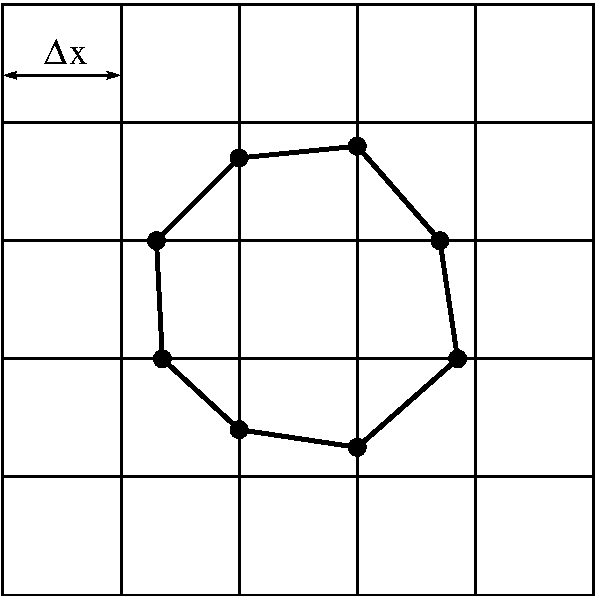
\includegraphics[width=0.45\textwidth]{fig_2a} &
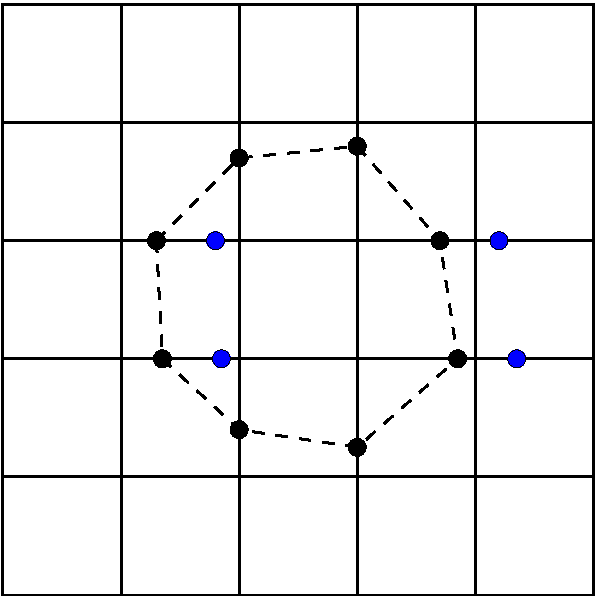
\includegraphics[width=0.45\textwidth]{fig_2b}\\
(a) & (b) \\[6pt]
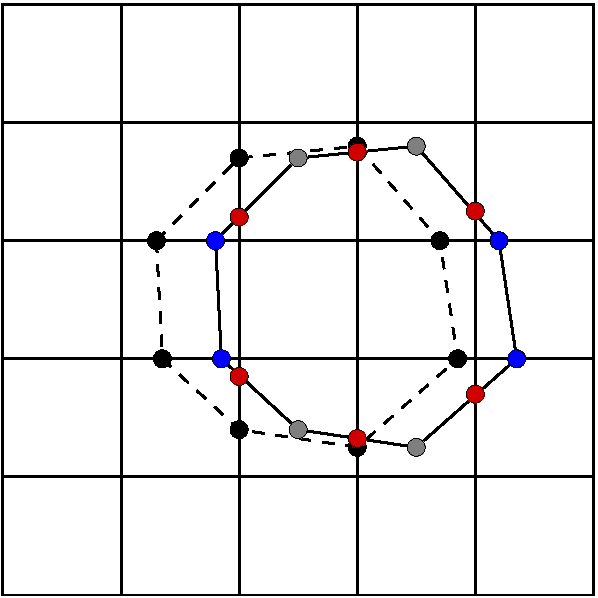
\includegraphics[width=0.45\textwidth]{fig_2c} &
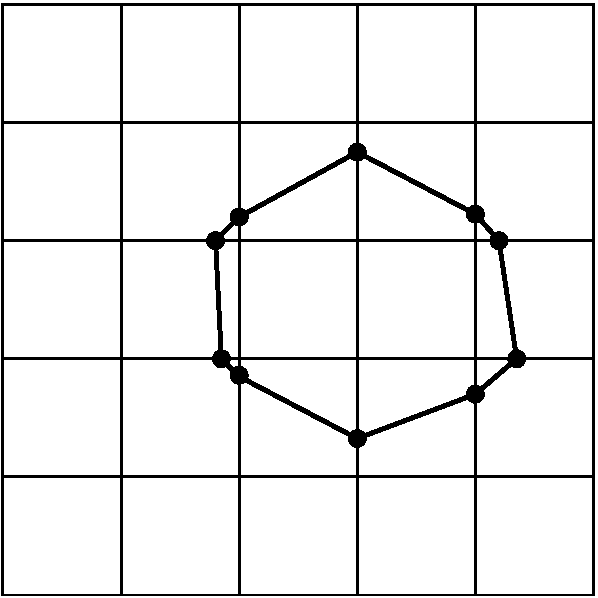
\includegraphics[width=0.45\textwidth]{fig_2d}\\
(c) & (d) 
\end{tabular}
\end{center}
\caption{One-dimensional advection of the EBIT method along
the $x$-axis: (a) initial interface line; (b) advection of
the markers on the grid lines aligned with the velocity component
(blue points); (c) advection of the unaligned markers (gray points)
and computation of the intersections with the grid lines (red points);
(d) interface line after the 1D advection.}
\label{Fig_EBIT_advection}
\end{figure}
% ----------

In the EBIT method, the interface is represented by a set of marker points placed on the grid lines. In order to keep the markers on the grid lines, it is necessary to compute the intersection points between the interface line and the grid lines at the end of each advection step. The equation of motion for a marker point at position $\X_i$ is
% ----------
\begin{gather}
\frac{d \X_i}{dt} = \U_i
\label{Eq_marker}
\end{gather}
% ----------
which is discretized by a first-order explicit Euler method
% ----------
\begin{gather}
\X^{n + 1}_i= \X^{n}_i + \U^{n}_i \Delta t
\label{Eq_marker_dis}
\end{gather}
% ----------
where the velocity $\U^{n}_i$ at the marker position $\X^{n}_i$ is calculated by a bilinear interpolation.

For a multi-dimensional problem, a split method is used to advect the interface (see Fig.~\ref{Fig_EBIT_advection}), which is similar to that described in \cite{Chirco_2022_95}, but with some improvements. The marker points placed on the grid lines that are aligned with the velocity component of the 1D advection are called \textit{aligned markers}, while the remaining ones are called \textit{unaligned markers}. Starting from the initial position at time step $n$, the new position of the aligned markers is obtained by Eq.~\eqref{Eq_marker_dis} (blue points of Fig.~\ref{Fig_EBIT_advection}b). To compute the new unaligned markers, we first advect them using again Eq.~\eqref{Eq_marker_dis}, obtaining in this way the gray points of Fig.~\ref{Fig_EBIT_advection}c. Finally, the new position of the unaligned markers (red points of Fig.~\ref{Fig_EBIT_advection}d) is obtained by a circle fit method which will be described in the next section.

% ----------
\begin{figure}
\begin{center}
\begin{tabular}{cc}
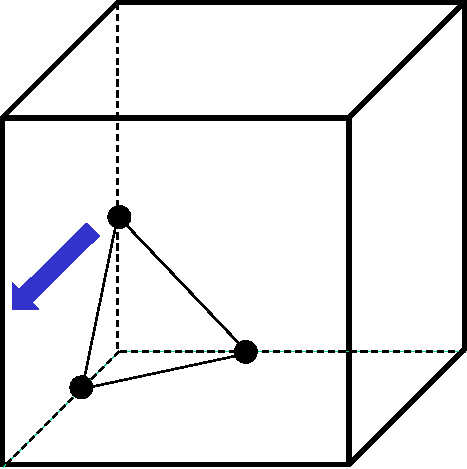
\includegraphics[width=0.45\textwidth]{EBIT_3d_a} &
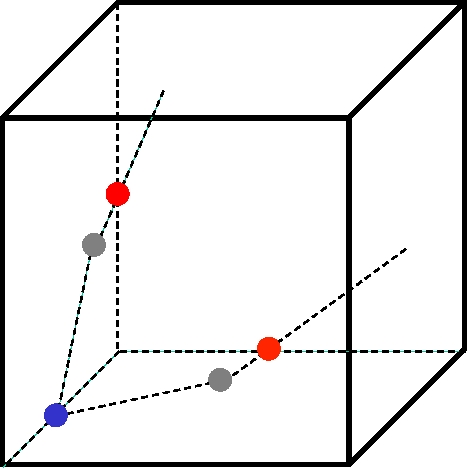
\includegraphics[width=0.45\textwidth]{EBIT_3d_b}\\
(a) & (b)
\end{tabular}
\end{center}
\caption{One-dimensional advection of the 3D EBIT method:
 (a) initial interface; (b) decomposition of the 3D advection problem.}
\label{Fig_EBIT_3D}
\end{figure}
% ----------

One important advantage of the split method is that it is relatively straightforward to extend the EBIT method to 3D. For the 1D advection along a coordinate direction of Fig.~\ref{Fig_EBIT_3D}a, the problem can be decomposed into simpler 2D problems on the two cell faces of Fig.~\ref{Fig_EBIT_3D}b, containing the advection direction under consideration and the marker points. In this way we can use most of the algorithms and routines we have developed for the interface advection in 2D. The detailed description of the 3D algorithm and the numerical tests will be presented in a future paper.

\subsection{Circle fit}

% ----------
\begin{figure}
\centering
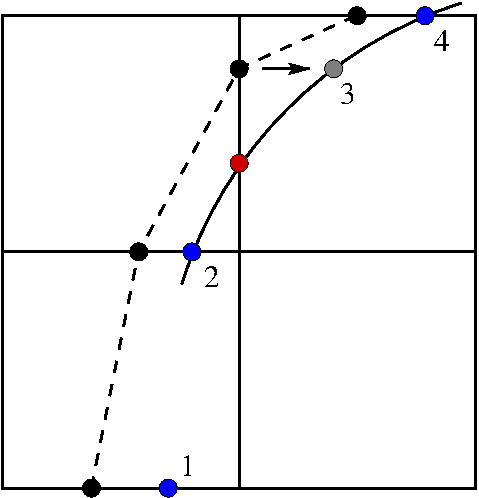
\includegraphics[scale=0.8]{fig_3}
\caption{Circle fit to compute the position of the unaligned marker (red point).}
\label{Fig_circle_fit}
\end{figure}
% ----------

In our previous paper about the EBIT method \cite{Chirco_2022_95}, we showed that the computation of the new position of the unaligned markers with a straight line fit was leading to poor accuracy of mass conservation, in particular at low spatial resolution. In this paper, we propose a circle fit as a method to improve the accuracy of mass conservation.
The new position of the unaligned marker (red point of Fig.~\ref{Fig_circle_fit}) is obtained by fitting a circle through the surrounding marker points and by computing its intersection with the corresponding grid line. The gray point is then discarded.
Whenever it is possible, we consider two circles for the fitting, through points 2,3,4 and 1,2,3 of Fig.~\ref{Fig_circle_fit}, respectively. In that case, the final position of the unaligned marker will be the average of the two intersections.


\subsection{Color Vertex}

% ----------
\begin{figure}
\centering
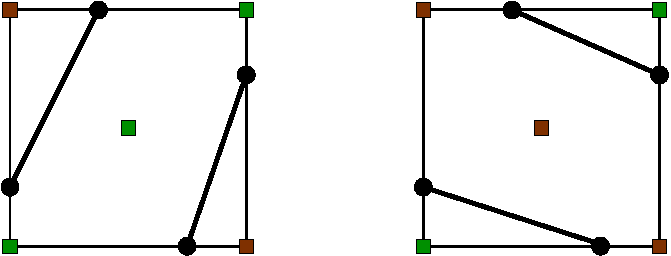
\includegraphics[width=\textwidth]{fig_4}
\caption{Two color vertex configurations (brown and green squares) to select a different connectivity 
in the same set of markers.}
\label{Fig_color_vertex}
\end{figure}
% ----------

In the EBIT method, the connectivity of the markers is implicit. When there are only two markers on the cell boundary, the interface portion in that cell is given by the segment connecting these two points. However, when there are four markers on the boundary, there are two possible alternative configurations, as shown in Fig.~\ref{Fig_color_vertex}. In order to select one of the two configurations without any ambiguity, we consider a technique called Color Vertex, which was first proposed by Singh and Shyy \cite{Singh_2007_224}, to implement an automatic topology change. The value of the Color Vertex indicates the fluid phase in the corresponding region within the cell, and five color vertices (four in the corners and one in the center of the cell) are enough to select one of the two configurations of Fig.~\ref{Fig_color_vertex}. In other word, we can establish a one-to-one correspondence between the topological configuration and the value of the color vertices within each cell, and then reconstruct the interface segments with no ambiguity.

Furthermore, the direction of the unit normal to the interface can also be determined based on the Color Vertex distribution. The local feature of the Color Vertex makes the EBIT method more suitable for parallelization, when it is compared to the data structure that is used for storing the connectivity in traditional Front-Tracking methods.

% ----------
\begin{figure}
\centering
\begin{subfigure}[b]{\textwidth}
\centering
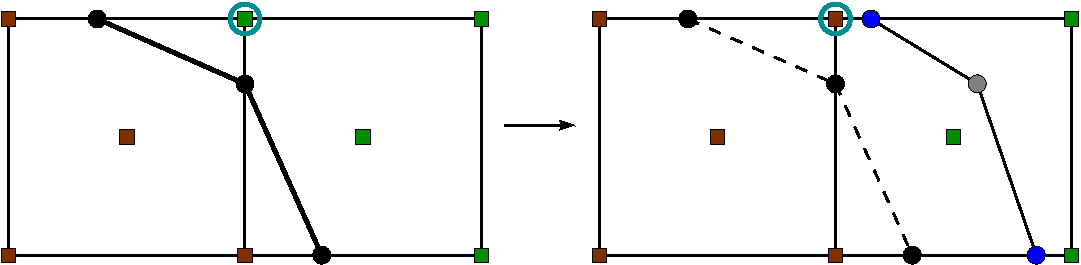
\includegraphics[width=\textwidth]{fig_5}
\end{subfigure}
\caption{Update of the Color Vertex value on a cell corner: its value changes, 
from green to brown, as the marker is advected across the grid lines intersection.}
\label{Fig_color_vertex_update_corner}
\end{figure}
% ----------

% ----------
\begin{figure}
\centering
\begin{subfigure}[b]{\textwidth}
\centering
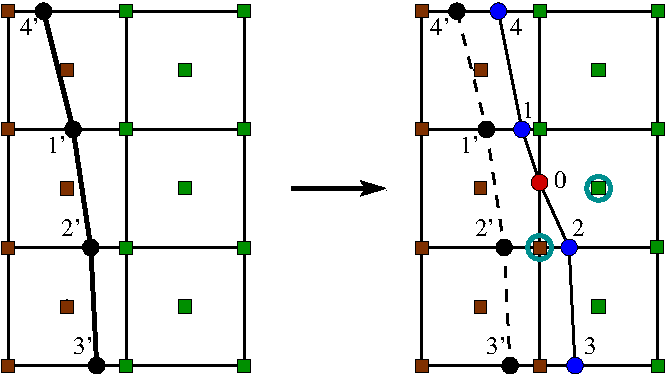
\includegraphics[width=\textwidth]{fig_6a}
\caption{}
\label{Fig_color_vertex_update_central_1}
\end{subfigure}
\\[10pt]
\begin{subfigure}[b]{\textwidth}
\centering
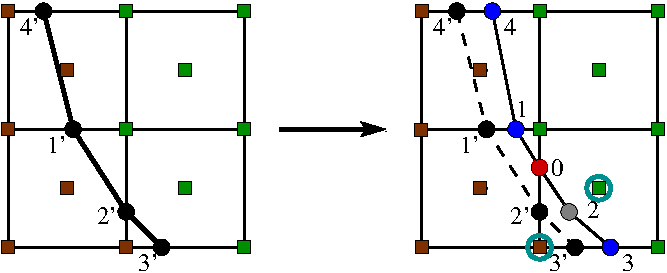
\includegraphics[width=\textwidth]{fig_6b}
\caption{}
\label{Fig_color_vertex_update_central_2}
\end{subfigure}
\caption{Update of the Color Vertex value in the cell center with an unaligned marker (red point).}
\label{Fig_color_vertex_update_central}
\end{figure}
% ----------

As the interface is advected, the value of a Color Vertex should also be updated 
accordingly to ensure that the implicit connectivity information is retained. For a Color Vertex located on a cell corner, we have to change its value if a marker moves across the intersection of the corresponding grid lines, as shown in 
Fig.~\ref{Fig_color_vertex_update_corner}.

In the present implementation of the EBIT algorithm the Color Vertex in the cell center 
is only used to select one of the two configurations shown in Fig.~\ref{Fig_color_vertex}. 
It is important to realize that in such a configuration, regardless of the direction of the advection, there are both aligned markers and unaligned ones.
Therefore, the algorithm for updating the Color Vertex in the cell center proceeds as follows (see Fig.~\ref{Fig_color_vertex_update_central}):

(1) If in the cell under investigation, after the interface advection there is an unaligned marker (red point 0 of Fig.~\ref{Fig_color_vertex_update_central}), we identify the interface segment through points 1 and 2 that brackets the unaligned marker and the corresponding segment through points 1' and 2', before the advection step. These two points are on opposite sides in Fig.~\ref{Fig_color_vertex_update_central_1} and on consecutive
sides in Fig.~\ref{Fig_color_vertex_update_central_2}.

(2) From the connectivity information before the advection step, we identify two more markers, points 3' and 4', that are connected to the segment 1'-2' on opposite sides,
and compute their new positions 3 and 4 after the advection step.

(3) If the four points 1, 2, 3 and 4 are unaligned markers, we do not need to update the value of the Color Vertex in the center, because in this case it is impossible to have an ambiguous configuration.

(4) We check if in the cell under investigation there is an aligned marker (point 2 in Fig.~\ref{Fig_color_vertex_update_central_1} and point 3 in Fig.~\ref{Fig_color_vertex_update_central_2}).

(5) If an aligned marker has been found, we identify the cell corner (bottom left corner of Fig.~\ref{Fig_color_vertex_update_central}) isolated by the segments connecting this marker and the new unaligned marker (point 0 of Fig.~\ref{Fig_color_vertex_update_central}). The value of the Color Vertex in the cell center is set to the opposite value of that of the cell corner.

With these simple rules, the value of the Color Vertex in the cell center is set to the correct value to select one of the two configurations of Fig.~\ref{Fig_color_vertex}.


\subsection{Topology change}

% ----------
\begin{figure}
\centering
\begin{subfigure}[b]{\textwidth}
\centering
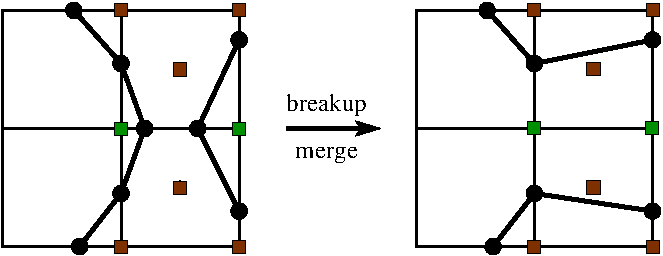
\includegraphics[width=\textwidth]{fig_7}
\label{Fig_topo_change_2}
\end{subfigure}
\caption{Topology change mechanism.}
\label{Fig_topo_change}
\end{figure}
% ----------

The topology change is controlled by the Color Vertex value distribution in an automatic manner. In the present implementation of the EBIT method, a marker point is present on a cell edge only if the value of the Color Vertex at the two edge endpoints is different. 

Furthermore, only one marker is allowed on a cell edge. When two markers move into the same edge, as shown in Fig.~\ref{Fig_topo_change}, they both will be eliminated automatically, because the value of the Color Vertex at the corresponding endpoints is the same, hence there cannot be any marker on that edge. 
Moreover, the ``surviving'' markers within the cell will be reconnected automatically, see again Fig.~\ref{Fig_topo_change}. This reconnection procedure enables ligament breakup or droplet merging in an automatic way during the interface advection. As a direct consequence of this procedure, the volume occupied by the reference phase can decrease or increase. In particular, it tends to remove droplets or bubbles which are smaller than the grid size. 

This topology change mechanism only affects interfaces that are approaching each other along a direction parallel to the grid lines. Because of the presence of a Color Vertex in the cell center, interfaces approaching along a diagonal direction do not induce any topology change, as long as the four markers remain on a different edge, as shown in Fig.~\ref{Fig_color_vertex}. Compared to the scheme depending on the tetra-marching procedure in Yoon's \cite{Yoon_2010_08} LCRM and Shin's \cite{Shin_2011_230} LFRM, this mechanism results in a more symmetric topology change.

However, in our method approaching interfaces along diagonal directions behave
differently from those approaching along parallel ones. A possible solution to this problem would be removing the restriction on the number of markers per edge, which would also allow us to capture the sub-grid scale interfacial structure and to control the topology change based on a physical mechanism. 


\subsection{Governing equations}

The Navier--Stokes equations for incompressible two-phase flow with immiscible fluids written in the one-fluid formulation are
% ----------
\begin{gather}
\frac{\partial \rho}{\partial t}
+ \U \cdot \nabla \rho= 0 \\
\frac{\partial \rho \U}{\partial t}
+ \nabla \cdot (\rho \U\U) = 
-\nabla p + \nabla \cdot \left[ \mu \left( \nabla \U + \nabla \U^T\right) \right] + \rho \G + \F
\label{Eq:NS}
\\
\nabla \cdot \U = 0
\end{gather}
% ----------
\noindent where $\rho$ and $\mu$ are density and viscosity, respectively. The gravitational force is taken into account with the $\rho \G$ term. Surface tension is modeled by the term $\F = \sigma \kappa \N \delta_S$, where $\sigma$ is the surface tension coefficient, $\kappa$ the interface curvature, $\N$ the unit normal and $\delta_S$ the surface Dirac delta function. 

The physical properties are calculated as
% ----------
\begin{gather}
\rho = H \rho_1 + (1 - H) \rho_2, \qquad \mu = H \mu_1 + (1 - H) \mu_2
\label{Eq:physical}
\end{gather}
% ----------
where $H$ is the Heaviside function, which is equal to 1 inside the reference phase and 0 elsewhere.

Since the markers are located on the grid lines, we consider a simple strategy to couple the EBIT method with the Navier--Stokes equations. From the position of the marker points and the value of the Color Vertices in the cell under investigation, we can easily compute the equation of the straight line connecting the markers and then the volume fraction $C$ \cite{Scardovelli00}. The volume fraction field is used to approximate the Heaviside function in Eq.~\eqref{Eq:physical}, to calculate the curvature by the generalized height function method \cite{Popinet_2009_228} and the Dirac delta function in Eq.~\eqref{Eq:NS}.

The numerical implementation of the EBIT method has been written in the Basilisk C language \cite{Popinet_2003_190, Popinet_2009_228}, which adopts a time-staggered approximate projection method to solve the incompressible Navier--Stokes equations on a Cartesian mesh or a quad/octree mesh. 
The Bell-Colella-Glaz (BCG) \cite{Bell_1989_85} second-order scheme is used to discretize the advection term, and a fully implicit scheme for the diffusion term. A well-balanced Continuous Surface Force (CSF) method is used to calculate the surface tension term \cite{Popinet_2009_228, Popinet_2018_50}.

The geometrical PLIC-VOF scheme generalized for the quad/octree grid \cite{Popinet_2009_228} in Basilisk is used to obtain the results for the comparisons of Sect. \ref{Numerical results and discussion}. The volume fraction $C$ is advanced in time with the following advection equation
% ----------
\begin{gather}
\frac{\partial C}{\partial t} + \U \cdot \nabla C  = 0
\label{Eq:PLIC-VOF}
\end{gather}
% ----------
The split scheme proposed by Weymouth and Yue \cite{Weymouth_2010_229} is used to discretize Eq.~\eqref{Eq:PLIC-VOF}. For a two-dimensional problem, the split scheme for the volume fraction advection, here first along the $x$-direction and then along $y$, is
% ----------
\begin{gather}
\frac{C_{i, j}^ {*} - C_{i, j}^{n-1/2}}{\Delta t} + \frac{\phi_{i + 1/2, j}^{n -1/2} - \phi_{i - 1/2, j}^{n - 1/2}}{\Delta} = C_c \frac{u_{i + 1 / 2, j}^{n} - u_{i - 1 / 2, j}^{n}}{\Delta}
\label{spl1}\\
\frac{C_{i, j}^ {n + 1/2} - C_{i, j}^{*}}{\Delta t} + \frac{\phi_{i, j + 1 / 2}^{*} - \phi_{i, j - 1 / 2}^{*}}{\Delta} = C_c \frac{v_{i, j + 1 / 2}^{n} - v_{i, j - 1 / 2}^{n}}{\Delta}
\label{spl2}\\
C_c = \begin{cases}
      1, & \text{if}\ C_{i, j}^{n - 1 / 2} > 0.5 \\
      0, & \text{if}\ C_{i, j}^{n - 1 / 2} \leq 0.5
\end{cases}
\label{Eq:PLIC-VOF_dis}
\end{gather}
% ----------
where $\phi_{i + 1/2, j}$ is the volume flux of the reference phase through the right cell face and $\Delta$ the grid spacing. The right-hand-side of Eqs. (\ref{spl1},\ref{spl2}) represents a compression or expansion term, since each component of the velocity field is not divergence-free. The step function $C_c$ is used to guarantee exact mass conservation for a multi-dimensional problem.

\subsection{Adaptive mesh refinement (AMR)}

% ----------
\begin{figure}
\centering
\begin{subfigure}[b]{0.8\textwidth}
\centering
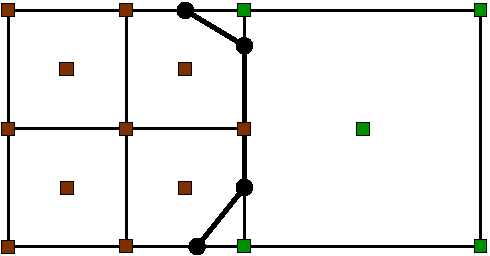
\includegraphics[width=\textwidth]{fig_8}
\end{subfigure}
\caption{The EBIT method with AMR.}
\label{Fig_ebit_amr}
\end{figure}
% ----------

An efficient adaptive mesh refinement (AMR) technique, which is based on a wavelet decomposition \cite{Popinet_2015_302} of the specified field variables, is implemented in Basilisk, which allows the solution of the flow field at high resolution only in the relevant parts of the domain, reducing in this way the computational cost of the simulation. 

Due to the restriction on the number of markers on each edge, the mesh refinement near the interface should be handled carefully. For the particular situation where the cells on the two sides of the interface are on different levels, as in Fig.~\ref{Fig_ebit_amr}, there are two markers on the same edge of the grid cell on the right. This instance violates the basic restriction of the current implementation of the EBIT method, and it is not allowed.

To avoid this inconsistency, we consider a simple strategy, that is to refine the cells within the $3 \times 3$ stencil of each interfacial cell to the maximum allowable level. With this assumption and the timestep limitation due to the maximum allowable $CFL$ number, which is equal to 1, in the EBIT method, the interface will not be advected between two grid cells at different resolution levels. In principle, this refinement strategy should be less efficient than that based on curvature, however the numerical results of the next section show that the efficiency is still comparable to that based on curvature when other criteria of refinement, such as velocity gradients, are introduced into the AMR strategy.

